\documentclass[preprint,aps,nofootinbib,a4paper,superscriptaddress,longbibliography,amsfonts,amssymb,amsmath,titlepage]{revtex4-2}
\usepackage{IEEEtrantools}
\usepackage{microtype}
\usepackage[toc,title,page,titletoc]{appendix}
%\usepackage[pdftex]{hyperref}
\usepackage{amsmath}
\usepackage{amsthm}
\usepackage{mathrsfs}
\usepackage{enumitem}
\usepackage[T1]{fontenc}
\usepackage{xfrac}
\usepackage{lmodern}
\usepackage[a4paper]{geometry}
\usepackage{hyperref}
\usepackage{mathbbol}


\newtheorem{definition}{Definition}

\begin{document}
\title{Tennis match forecasting; how AI can beat book makers on their own platforms}

\author{Patrick Schall}
\email{patrick.schall@gmail.com}

\author{Vahid Toomani}
\email{vahidtoomani2002@gmail.com}

\date{\today}

\maketitle
\tableofcontents

\newpage

\section{Introduction}

In 1943, Walter Pitts and Warren McCulloch laid the foundation for artificial intelligence (AI) and its subfield, machine learning, with their first mathematical model of a neural network.

Seven years later, Alan Turing posed the fundamental question: ``Can machines think?'' He developed the Turing test, originally known as the imitation test, which assesses whether a machine exhibits intelligent behavior. In his seminal work ``Computing Machinery and Intelligence'' (1950), Turing didn’t settle for a simple definition of machines or thinking; instead, he asked a more profound question: ``Can machines do what we, as thinking entities, can do?''

Over the past 70 years, fueled by ever-growing computational power, increased storage capacity, and an exponentially expanding pool of data, machine learning (ML) and deep learning algorithms have revolutionized the field of data science. ML models can predict whether a customer will cancel their contract with a telecommunication provider, determine the authenticity of an unknown painting, verify the origin of wine analyzed in a laboratory, and even classify tumors as benign or malignant. Recent breakthroughs include autonomous driving cars, defeating the world’s best Go player (a game more complex than chess and reliant on intricate pattern recognition), and predicting the 3D structure of proteins from their amino acid sequences (AlphaFold 2).

One significant advantage of machine learning models lies in their ability to forecast the future with a high degree of certainty. Today, ML models are employed to predict weather patterns, estimate fuel consumption for new cars, and optimize maintenance intervals for machinery. A practical application of ML is in the prediction of sports betting outcomes. By analyzing historical data, player performance, and other relevant factors, ML models can provide valuable insights for informed betting decisions.

In the following work, we aim to design a machine learning model, employing standard ML algorithms like Decision Tree, Random Forest, Support Vector Machine (SVM), and more advanced deep learning models like Convolutional Neural Network (CNN), capable of predicting the outcomes of tennis matches played on the ATP tour. We aim to better understand which features influence the outcome of a tennis game. Additionally, we intend to develop a betting strategy that minimizes investment losses and maximizes return on investment by placing bets on the odds provided by two bookmakers: Bet365 and Pinnacle Sports. In general, we aim to develop a betting tool which:
%
\begin{enumerate}
\item Predicts tennis matches with high accuracy.
\item Yields a net plus when betting money on tennis matches on bet365.com and pinnacle.com
with their respective odds.
\end{enumerate}
%
This work, carried out by Vahid Toomani with a scientific background in math and physics, and Patrick Schall with a scientific background in molecular biology, will not only assist gamblers in maximizing their ROI and aid bookmakers in improving their odds, but it will also help tennis players and their coaches better understand the main features influencing the outcome of a tennis game.

\subsection{International tournaments and book makers}
ATP, Pinnacle sports, Bet 365

\subsection{Elo system}
Elo rate

\subsection{objectives}
Goals
\begin{itemize}
\item What are the main objectives to be achieved? Describe in a few lines.
\item For each member of the group, specify the level of expertise around the problem addressed?
\item Have you contacted business experts to refine the problem and the underlying models? If yes, detail the contribution of these interactions.
\item (Are you aware of a similar project within your company, or in your entourage? What is its progress? How has it helped you in the realization of your project? How does your project contribute to improving it?).
\end{itemize}

\section{Exploratory data analysis (EDA)}


\subsection{Data fetch}

Our initial data set consist of ATP matches from 2000 until 2018 fetched from \href{https://www.kaggle.com/datasets/edouardthomas/atp-matches-dataset}{Kaggle.com}. This Dataset is provided by Eduard Thomas to Kaggle.com. Since our initial data frame was fairly outdated and were missing a lot of odds for the years 2000 till 2003 we fetched new data from \href{http://tennis-data.co.uk/}{tennis-data} and deleted all the data with missing data for the odds. This resulted in a data frame consisting of data from 2004 until 2024.

\subsection{Data enrichment \& cleaning}
Which parts of data dropped or added?

\subsection{Data statistics and visualisations}
Put graphs and statistics of the data here, like \ref{ps-odds-dist}.
%
\begin{figure}[h]
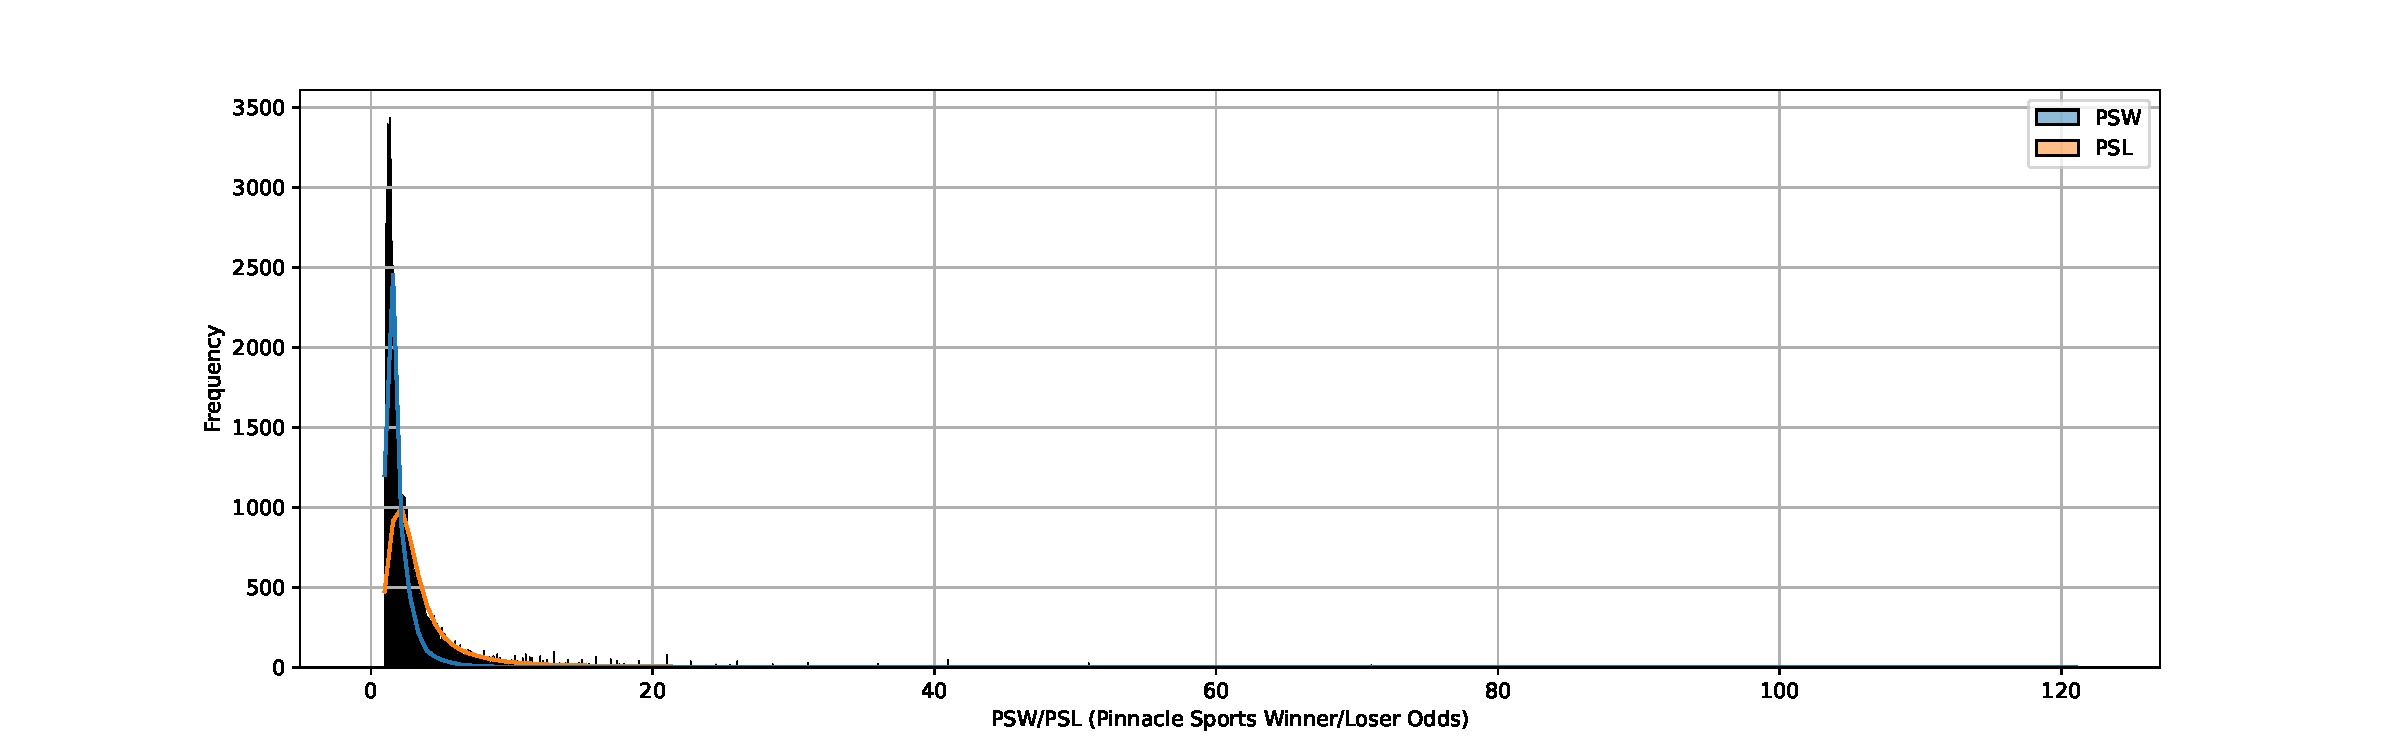
\includegraphics[width=\textwidth]{pictures/ps-odds-dist.pdf}
\caption{Distribution of Pinnacle Sports Winner/Loser Odds}
\label{ps-odds-dist}
\end{figure}
%
%
\begin{figure}[h]
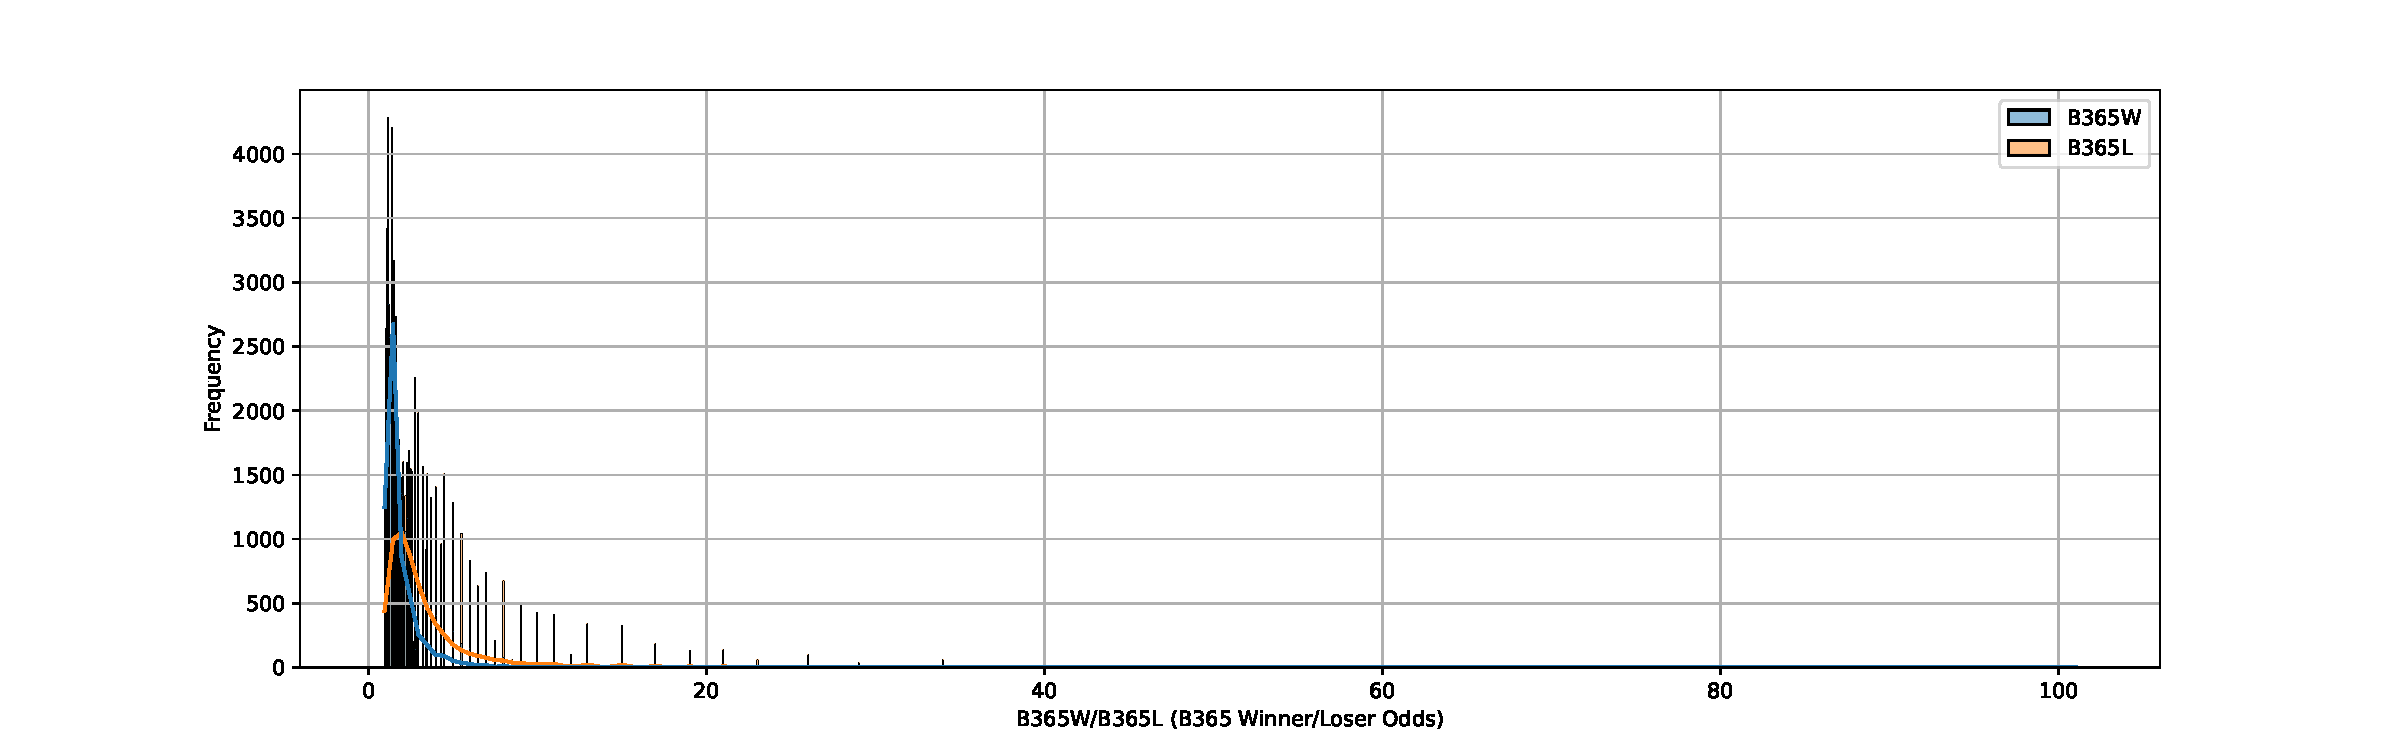
\includegraphics[width=\textwidth]{pictures/b365-odds-dist.pdf}
\caption{Distribution of B365 Winner/Loser Odds}
\label{b365-odds-dist}
\end{figure}
%
%
\begin{figure}[h]
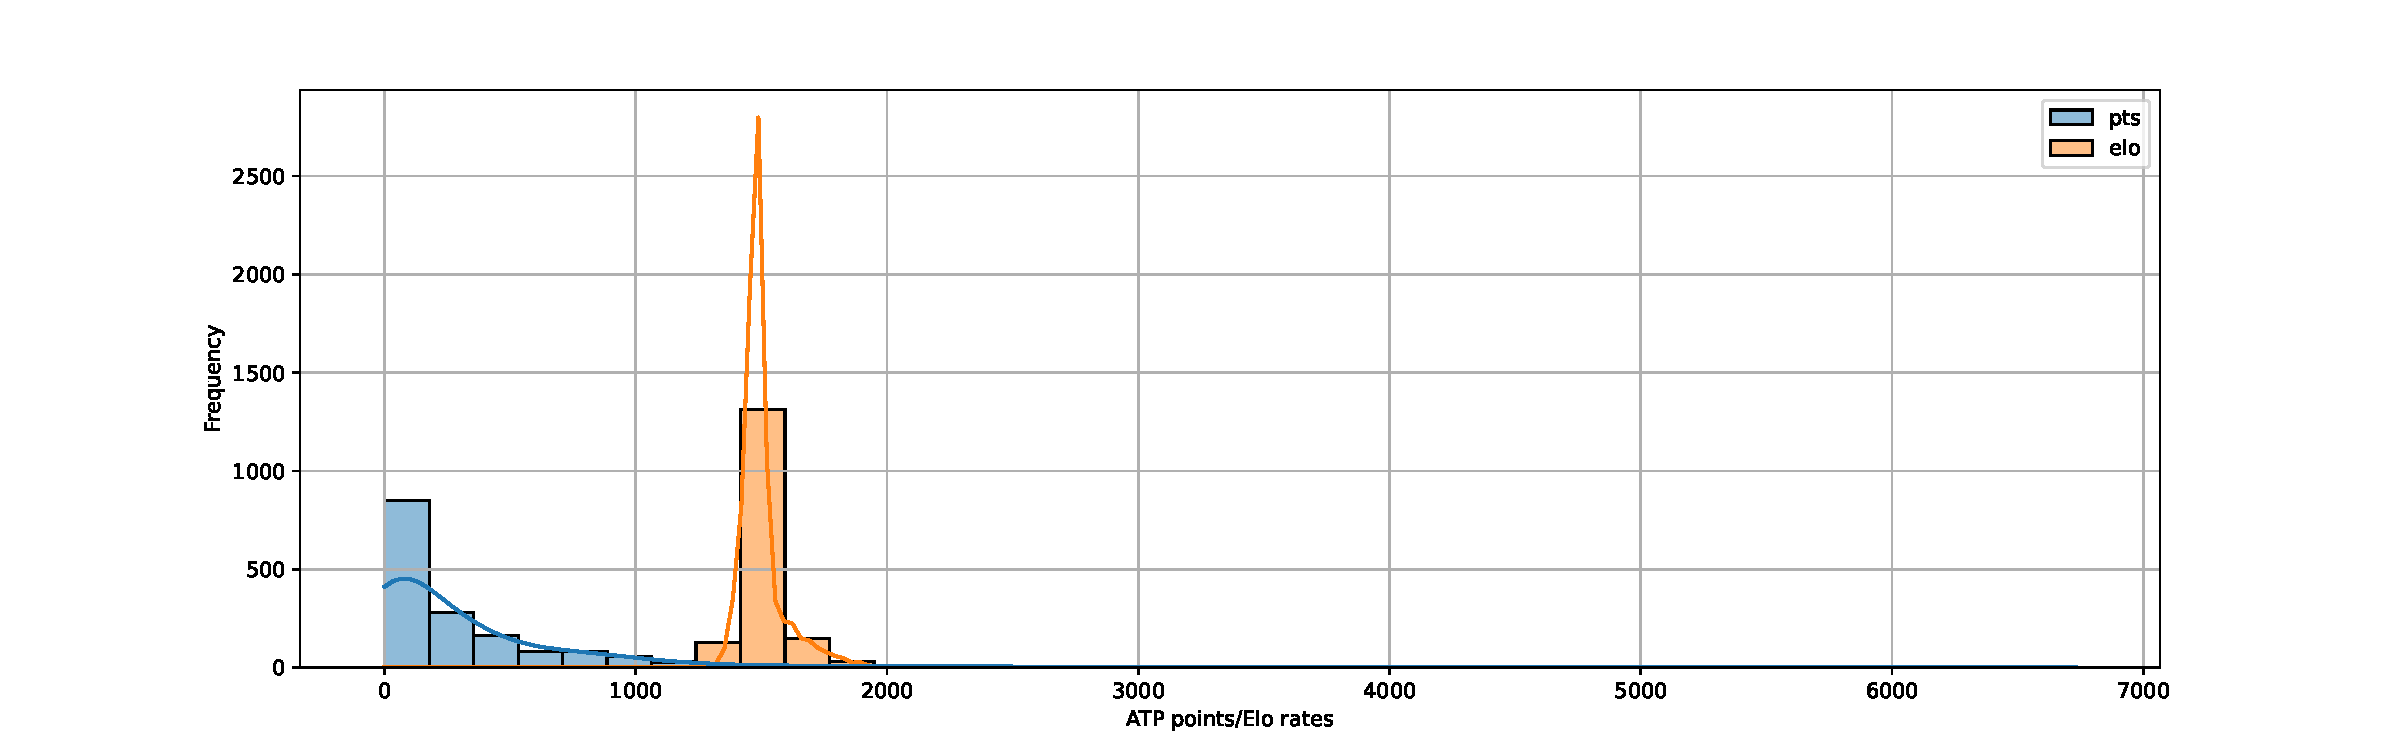
\includegraphics[width=\textwidth]{pictures/elo-rates-atp-point-dist.pdf}
\caption{Distribution of elo rates and atp points}
\label{elo-rates-atp-point-dist}
\end{figure}
%
%
\begin{figure}[h]
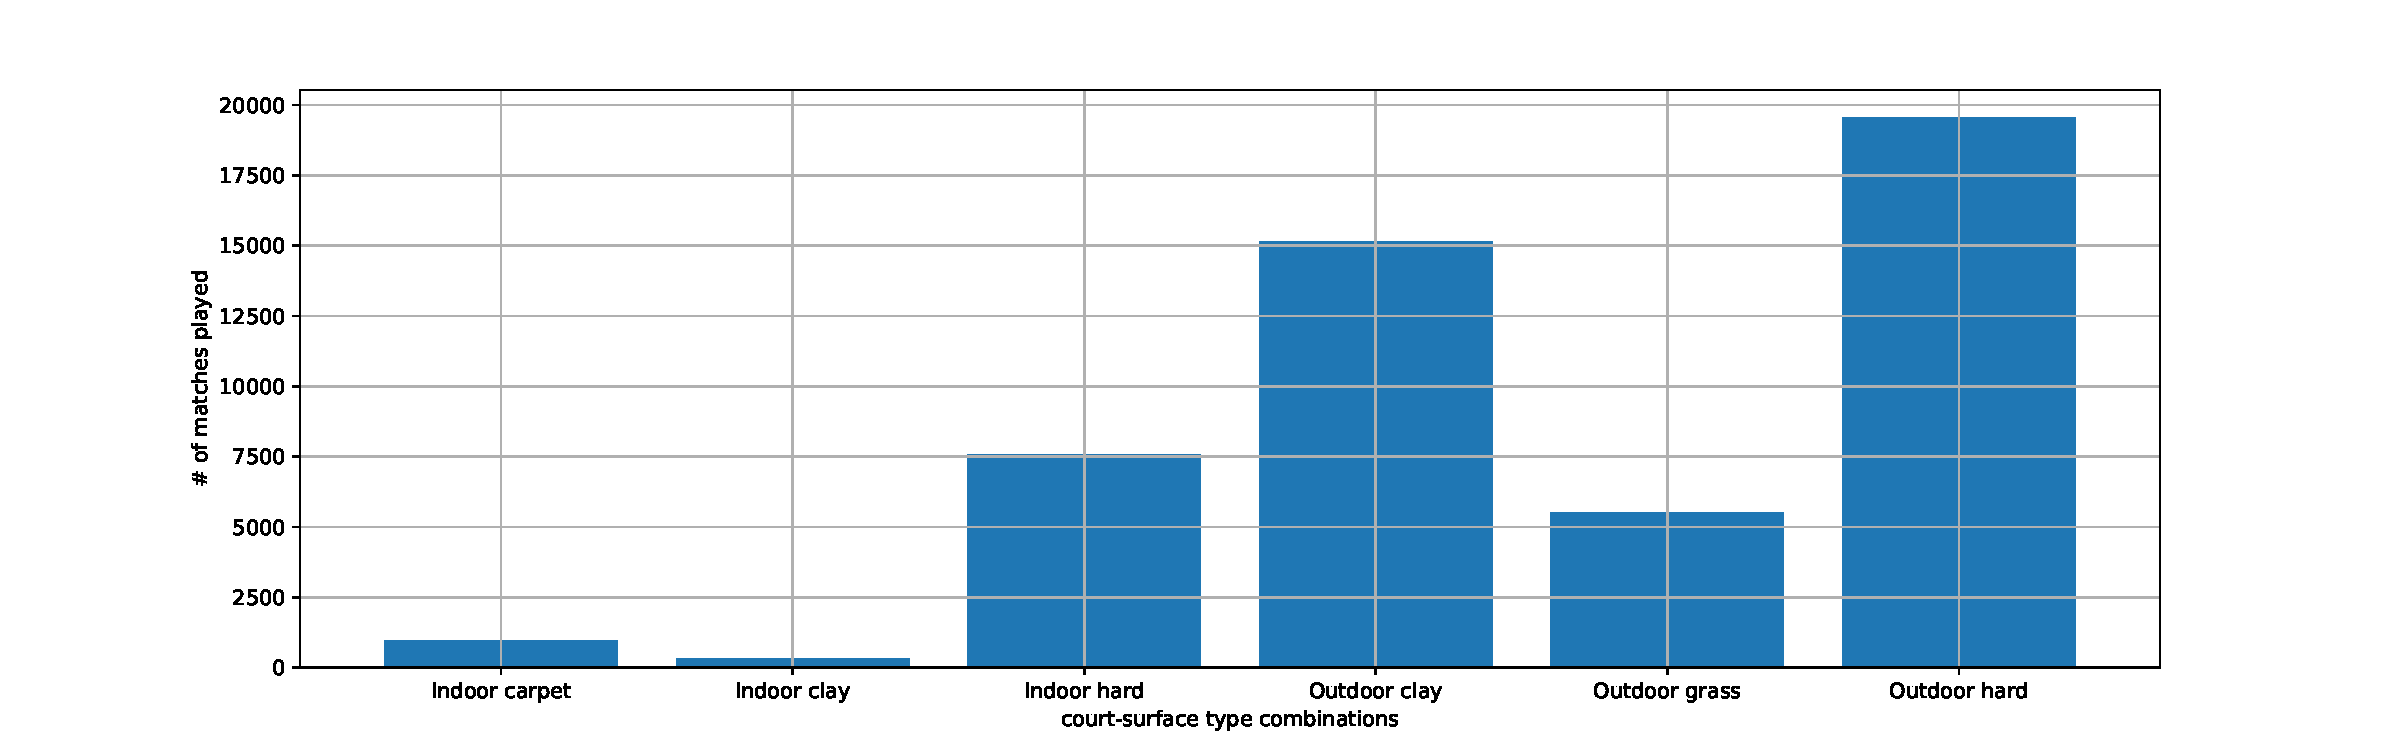
\includegraphics[width=\textwidth]{pictures/match-count-field-type-dist.pdf}
\caption{Distribution of Pinnacle Sports Winner/Loser Odds.}
\label{match-count-field-type-dist}
\end{figure}

\subsection{Strategies}
Strategies

\subsection{Feature selection}

\section{ML models and learning}


\subsection{Model selection}


\subsection{Random forest}


\subsection{Ada boost}


\subsection{Support vector Mmachine}


\subsection{Voting}


\subsection{Dense neural network}

\section{Post learning analysis \& packaging}


\subsection{Uncertainty cutoff}


\subsection{Cutoff optimization}


\section{Conclusion}

%\begin{thebibliography}{9}
%\bibitem{Aksteiner:2016mol}
%S.~Aksteiner and T.~B\"ackdahl,
%``Symmetries of linearized gravity from adjoint operators,''
%J. Math. Phys. \textbf{60} (2019) no.8, 082501
%doi:10.1063/1.5092587
%[arXiv:1609.04584 [gr-qc]].
%\end{thebibliography}
\end{document}